\section{Real-World Configuration Changes}
\label{sec:study}

This section describes a preliminary study to investigate whether
and how configuration changes arise during software evolution.
%\todo{say the object is whether such changes
%often exist in practice?}
\todo{perphas the study purpose should be toned down a bit. donot
claim too much. just say whether configuration changes are frequent or not.}

In the software engineering literature, desipte a rich body of
software change analysis work, 
software configuration changes across multiple
versions are less studied.
Knowing whether and how configuration options evolve in practice
can be beneficial for both software developers
and tool designers. For example, knowing what types
of configuration changes are common in practice
can help developers improve the current designs and
implementations to create better systems or documentations
; for tool builders, so that they can improve their tools
to match reality (e.g., by knowing the types of configuration
changes that occur most frequently).


\begin{table}[t]
\vspace{1mm}
\centering
\small{
\setlength{\tabcolsep}{.40\tabcolsep}
\begin{tabular}{|l||c|c|c|c|}
\hline
 Program & Versions & Years & LOC (latest version)  & Language\\
 \hline
 \hline
 MySQL & 5.1, 5.5, 5.6, 5.7 & 3 && C/C++\\
 Apache& 2.0, 2.2, 2.4 & 3  & &C/C++\\
 FireFox& 7.0--22.0 (16 versions) & 3  & &C/C++\\
 Randoop & 1.2.1, 1.3.2, 1.3.3 & 6 &    &Java\\
 Weka & 3.4, 3.5, 3.6, 3.7  & 2  &  &Java\\
 JChord & 1.0, 2.0, 2.1 &  4 &   &Java\\
 Synoptic & 0.04, 0.05, 0.1 & 2   & &Java\\
 JMeter & 2.6, 2.7, 2.8, 2.9& 2   & &Java\\
\hline
\end{tabular}
}
\vspace{-2mm}
\Caption{{\label{tab:subjects} The open-source
software systems we studied and their characteristics.
Column ``Years'' is the active development period
for the selected versions. 
}
}
\end{table}


\begin{table}[t]
\vspace{1mm}
\centering
\small{
\setlength{\tabcolsep}{.50\tabcolsep}
\begin{tabular}{|l||c|c|c|c|}
\hline
 Program & \#Added Options & \#Deleted Options& \#Modified Options\\
 %&  Options &  Options&  Options \\
 \hline
 \hline
 MySQL& 26 & 24 & 23 \\
 Apache & 5 & 0 & 10 \\
 FireFox& 28 & 7 & 56 \\
 Randoop & 37  & 26 & 2\\
 Weka &  72 & 4 & 13 \\
 JChord & 13  & 10 & 5 \\
 Synoptic & 3 & 0 & 2 \\
 JMeter & 17  & 3 &  12 \\
\hline
\hline
 Total & 201 & 70 & 123 \\
\hline
\end{tabular}
}
\vspace{-2mm}
\Caption{{\label{tab:options} The total number of new, deleted,
and modified configuration options for each subject program
in the studied versions.}
}
\end{table}


\begin{table}[t]
\vspace{1mm}
\centering
\small{
\setlength{\tabcolsep}{.50\tabcolsep}
\begin{tabular}{|c|c|}
\hline
 \textbf{Change Type} & \textbf{Description} \\
 \hline
 \hline
Bugs & Fix existing bugs\\
 \hline
Renaming & Change the original option name\\
 \hline
Features & Add, remove, or modify features\\
 \hline
Reliability & Improve reliability or performance\\
 %\hline
%Maintainance & Maintain the code and documentation \\
%& (e.g., renaming the option name) \\
\hline
\end{tabular}
}
\vspace{-2mm}
\Caption{{\label{tab:conftypes} Types
of configuration changes identified in our
study from the subject programs in Table~\ref{tab:subjects}.}
}
\end{table}

\begin{table}[t]
\vspace{1mm}
\centering
\small{
\setlength{\tabcolsep}{.50\tabcolsep}
\begin{tabular}{|l|c|c|c|c|}
\hline
 Program & \multicolumn{4}{|c|}{\textbf{\#Changed Configuration Options}} \\
 \cline{2-5}
 & Bugs & Renaming & Features & Reliability \\
 \hline
 \hline
 MySQL & 0 & 15 & 55 & 3 \\
 Apache& 0 & 0 & 11 & 4 \\
 FireFox& 28 & 0 & 55 & 8 \\
 %FindBugs & & & & \\
 Randoop & 0  & 2 & 62  & 1\\
 Weka & 1  & 0 & 81  & 8 \\
 JChord & 0  & 2 & 24 & 2\\ %add a default file
 Synoptic & 0 &  5 & 0 & 0\\
 JMeter & 7  & 0 & 18 & 7 \\
\hline
\hline
 Total & 36 & 24 & 301 & 33 \\
\hline
\end{tabular}
}
\vspace{-2mm}
\Caption{{\label{tab:categories} The numbers of configuration changes of
each type (Table~\ref{tab:conftypes}).}}
\end{table}


\subsection{Subject Programs and Study Methodology}

We investigate how software configuration evolves in
\studysubjnum open-source configurable systems, as listed
in Table~\ref{tab:subjects}. The \studysubjnum contains
three C/C++ software and six Java software.
MySQL~\cite{}  is a popular relational database management
system. Apache~\cite{} is a HTTP server which has acquired
the largest share on the internet since 1996. FireFox~\cite{}
is an open-source browser available on multiple platforms.
Randoop~\cite{} is an automated test generator for Java
programs. Weka~\cite{} is a toolkit that implements machine
learning algorithms. JChord~\cite{} is a program analysis platform that
enables users to design, implement, and evaluate static and
dynamic program analyses for Java. Synoptic~\cite{} mines a
finite state machine model representation of a system from
logs. JMeter~\cite{} is a tool to load test functional
behavior and measure performance.
Each program is highly configurable, and has evolved over
a long period of time (\todo{xx--xx} years).


In comparison to software bugs that have well-maintained
bug databases and have benefits from many
software bug characteristic studies~\cite{},
a configuration evolution study is much harder, mainly
because historical misconfigurations (due
to configuration changes) usually have not been
recorded rigorously in database. Usually, when
regression tests pass, developers may treat the
software behaviors have been validated. Therefore,
the description of software misconfigurations is user-driven,
the ``fixes'' may be recorded simply as pointers
to manuals and best-practice documents.

In our study, rather than searching bug repositories,
we manually examine the revision history of the subject programs
in the past XXX years, and searched for the related
keywords such as ``Added/Removed/Updated option'' in
in commit messages and in the change logs,
which records developers' activities
during software evolution. For each match,
we read the description of the change,
and the ``diff'' of the original file and the
changed file. This information indicated
to us whether the change affects how the
software should be configured to produce
the original behavior. We identifies the
changed code and its affected configuration options
manually.

The identified configuration changes by our methodology is certainly not complete.
Our methodology only studies changes that are directly made to options \todo{xxx}.
However, it is entirely possible that other
changes to the core logic code would also
 lead to reconfigure the software\todo{rephrase above}


\subsection{Findings}

Tables~\ref{tab:options} and~\ref{tab:categories}
summarize the study results.



\subsubsection{Characteristics}

We further classify configuration changes into
four categories (Table~\ref{tab:conftypes}) based
on the change purpose. Each change belongs to a single category.
Table~\ref{tab:categories} shows the number of
configuration change types for each subject program.
Feature related changes are the largest group across
all subject programs. These changes include
adding new configuration options to control \todo{xx}.
\todo{normal examples}

The following are options obsolete and have been removed in
MySQL 5.5. Where alternatives are shown, applications should
be updated to use them
\todo{need rephrase}

Other three categories of canges occur as well, although
with less frequency than the feature-related changes.
Except for changes to fix a reported, changes to rename
a configuration option and changes to improve
software reliability would also affect a
software's normal behaviors. For example,
\todo{example}


%\vspace{1mm}
%\noindent\textbf{Examples}



\begin{figure*}[t]
  \centerline{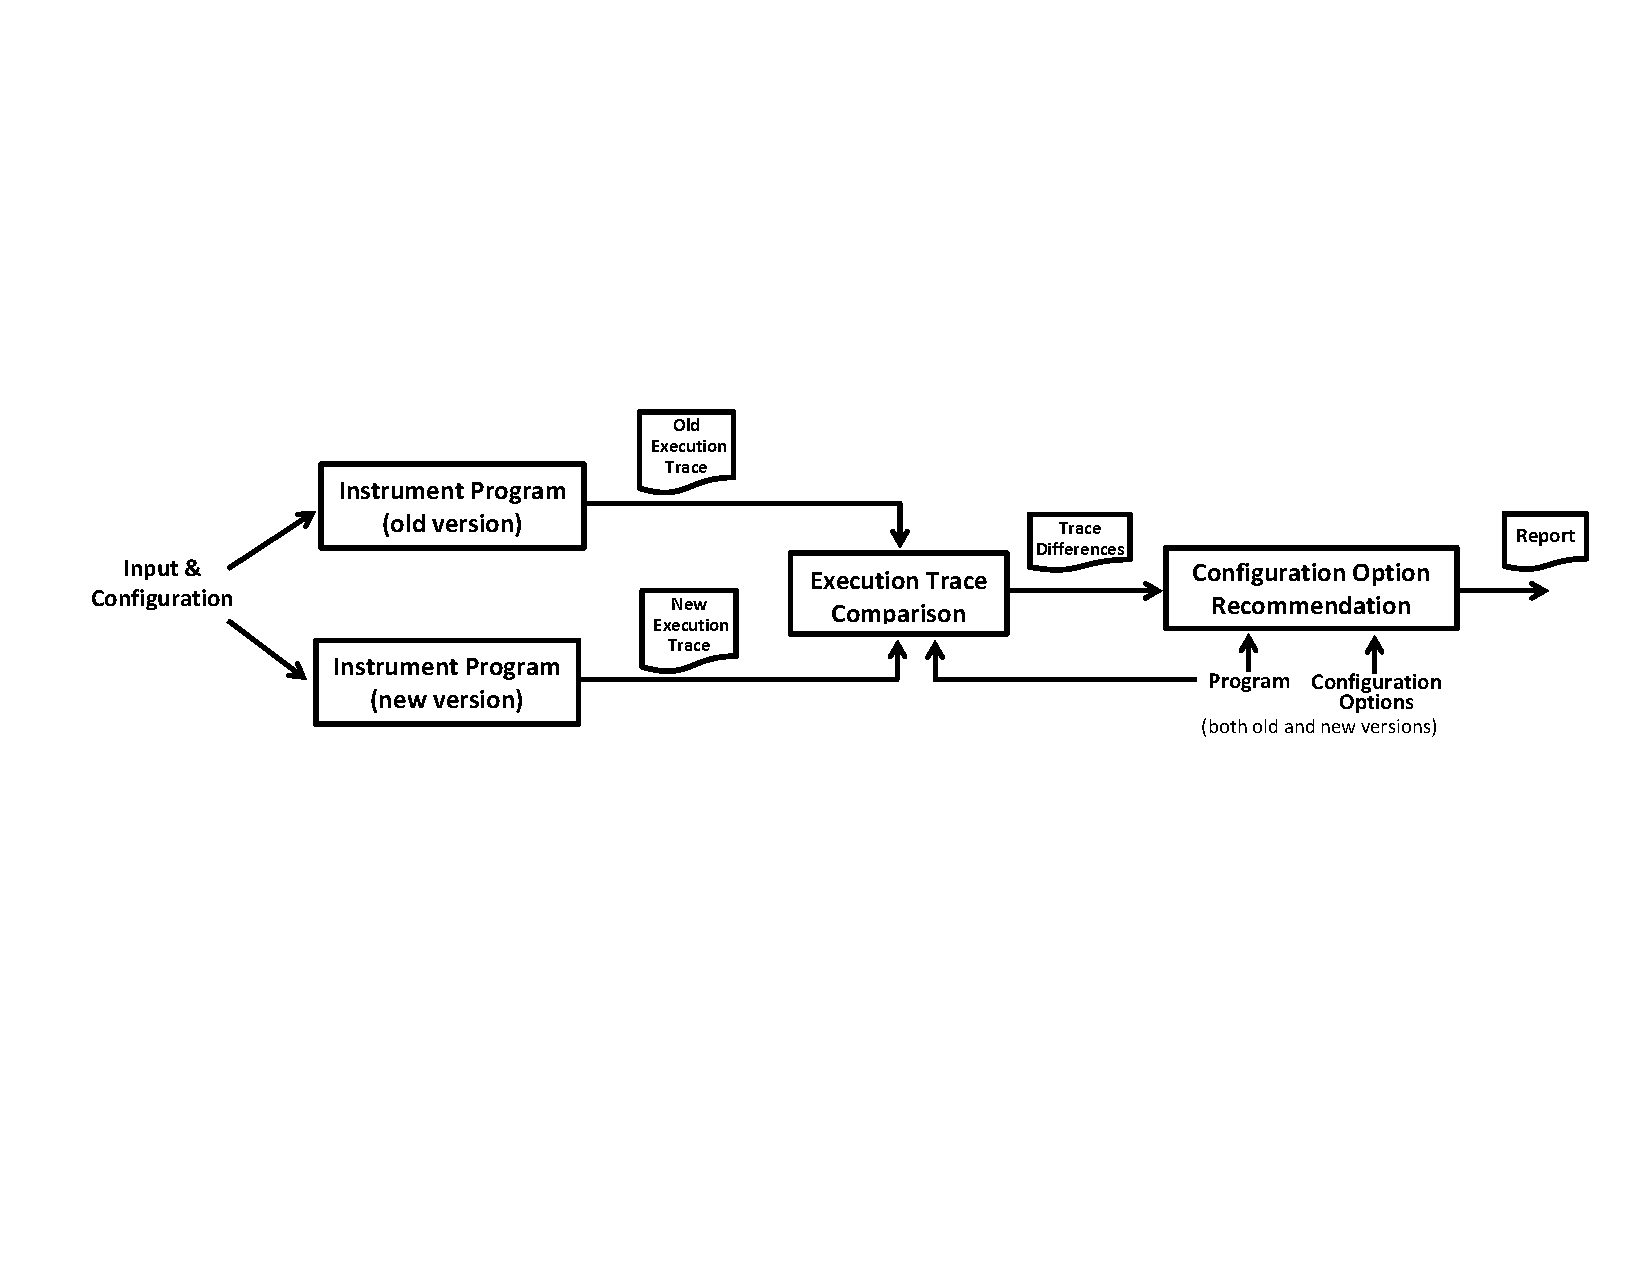
\includegraphics[scale=0.69]{workflow}}
  \vspace*{-2ex}\caption {{\label{fig:overview} The architecture of
  our \ourtool technique. The instrumented program versions and
  two execution traces are produced by the step in
  Section~\ref{sec:profiling}. 
  The ``Execution Trace Comparison'' step is described in
  Section~\ref{sec:comparison}. The ``Configuration Option Recommendation'' step
  is described in Section~\ref{sec:rootcause}.
}}
\end{figure*}


%\subsection{Summary}
\subsubsection{Implications}

Our study has three chief findings:
\textbf{(1)} configuration
changes arise frequently during software evolution: for
all subject programs we have studied, every version
includes configuration changes. \textbf{(2)} most configuration
changes fall into a small number of types, among
which \todo{most of them are feature related.}
and \textbf{(3)} a large number of
configuration changes may affect a program's
behaviors. Users must properly reconfigure a
program in order to maintain its original behavior.
\todo{rephrase above. the purpose is to
illustrate configuration change is prevalent}

Our study also indicates that configuration errors
can be frequent... \todo{xxx}
%\textbf{Implications.} If a user ignore the changes, even if the tests
%all pass. User-driven

\subsection{Threat to Validity}
Our study is limited by the open-source
software systems we chose, which may not reflect
the characteristics of other software systems.
We only examined software change logs to identify
changed configurations, which is a biased
subset; there may be (many) other configuration
options are affected by code changes. A similar
study that leverages the recent advance in
change impact analysis~\cite{} may be needed
to identify a more complete set of
configuration changes.
